\section{Oppsumering fra skype 13. August}
\begin{itemize}
\item
\textsc{GranFilm} produserer komplekse amplituder. Igjennom hoved-outputfilen gir det ut 
$\Delta R/R$ osv... Denne filen inneholder størrelsene som avhenger av den valgte polarisasjonen ('s'/'p').
Den gir også ut ''uoffisiell output''(eller hva nå enn Ingve sa) som inneholder data
som ikke koster noe spesielt ekstra å gi ut. Dataen fås ut ved å legge til et ekstra '-py' flag når 
man kjører \textsc{GranFilm} og lagres i en fil med samme navn som hoved-outputfilen men med en ekstra 
ende: '\_RefTrans'. Resultatene i denne filen er uavhengig av om valget du velger 's' eller 
'p' som input. Her ligger både $r_p$ og $r_s$ for de granulære overflatene, i tillegg til 
de samme størrelsene for en tilsvarende flat-overflate (altså uten sphærene) og kalles  
'r\_p fresnel' og 'r\_s fresnel'. OBS! Hver størrelse er gitt ved realdel og kompleks del.
\\
\\
Om jeg forstod Ingve riktig, er
disse størrelsene er amplitude-størrelser: Anta p-polarisert bølge med amplitude $E_i$, da er reflektert 
amplitude
\begin{align*}
E_r = r_p E_i
\end{align*}
og 
\begin{align*}
   E_r E_r^* &= r_p r_p^* E_i E_i^* \\
   |E_r|^2 &= |r_p|^2 |E_i^2|\\
   I_r &= R_p I_i
\end{align*}

\textbf{En annen viktig ting:} Anngående plotting og til plott til rapporten: 
\textbf{bruk større font! dette burde fikses med en gang.}


\item \textbf{Oppgaver:}
   Ta for deg et glass substrat (SiO$_2$), MgO eller alumna Al$_2$O$_3$ (et rent dielektrikum
   substrat som er temperatur uavhengig), vakuum rundt og termokromme sphærer (Se Figur \ref{fig:granular}).
   Bruk dataen i området $\sim 1$eV-4eV (den fra Kang 2012) som ditt termokromme materiale.
   \begin{figure}[h!]
     \centering
      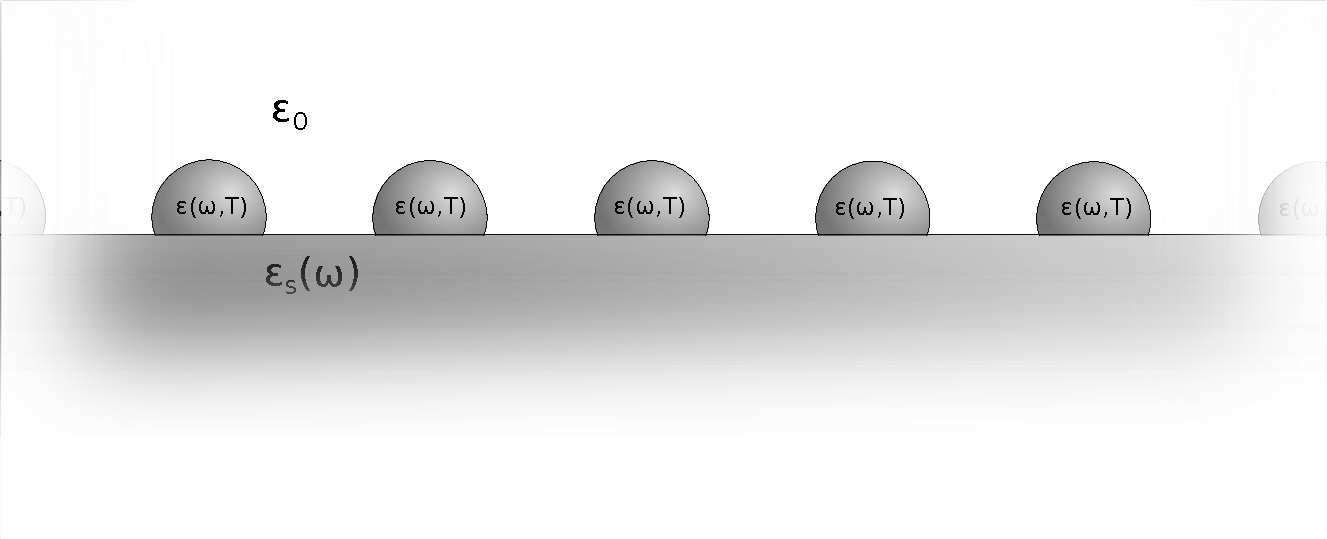
\includegraphics[width=0.5\textwidth]{granularFilm1.pdf}
      \caption{
      }
      \label{fig:granular}
   \end{figure}
   %
%\begin{lstlisting}[style=FormattedNumber, language=bash]
%\end{lstlisting}
   \begin{enumerate}
      \item
         \textbf{Sjekk at resultatene dine er fornuftige igjennom teorien for en flat overflate.}
         Altså, bruk de teoretiske fresnel koeffisientene for en flat overflate med dielektrisitet
         dataene dine og sammenlign dette med dataen du har fått ut fra \textsc{GranFilm}.

         \item
            \textbf{Plot $\Delta R/R$ for alle temperateurer gitt i Kang.} \\
            Her er litt informasjon om $\Delta R/R$:
            \begin{itemize}
               \item $\Delta R/R$ gir den relative endringen i $R$ i forhold til en flat overflate.

            \item Om den tynne filmen ikke oppfører seg annerledes enn en flat overflate
               vil $\Delta R/R$ være lik 0.
            \item Med andre ord, $Delta R/R$ gir bidraget fra de sphæriske kulene. ?Hvordan de kollektivt
               endrer refleksjonen. 
            \item Om $\Delta R/R > 0$ (positiv) bidrar den granulære filmen til større refleksjon.\\
               \\
            Om $\Delta R/R < 0$ (negativ) bidrar den granulære filmen en reduksjon av refleksjonen.
               \\
            $\Delta R/R = 1 \rightarrow $ dobbelt refleksjon sammenlignet med flat overflate.
               \\
            $\Delta R/R = 0 \rightarrow $ ingen forskjell fra flat overflate.

            \item resonanser $\rightarrow$ hvilken avhenger av $\varepsilon$

            \item Hvis det er mye ''dynamikk'' i denne dataen $\rightarrow$ da blir $\varepsilon$
               viktigere (??og motiverer neste oppgave??).
            \end{itemize}
         \item 
            For en gitt energi (f.eks E = 3.5 eV) vil du ha data for permittivitet $\varepsilon$
            for flere temperatuerer. 
            \textbf{Plot $\varepsilon(\omega,T)\big|_{\omega=\omega(3.5\text{eV})}$ 
            og sjekk om denne er forholdsvis glatt.} (altså plott permittivitet for gitt energi
            som funksjon av temperatur) Hvis ja kan denne
            dataen interpoleres med temperatur og gjøres for alle energier.
         \item
            \textbf{Interpoler den dielektriske dataen i energi og temperatur og prøv å lag et
            2D konturplot: et plott for Re$[\varepsilon]$ og et for Im$[\varepsilon]$.}
   \end{enumerate}
 



\end{itemize}
